\chapter{Das Problem des kürzesten Pfades}
\label{spp}
In diesem Abschnitt wird ein Einstieg in das Problem des kürzesten Pfades (engl. \textit{Shortest Path Problem}, SSP) gegeben. In vielen Bereichen lassen sich Pfadplanungsprobleme als Suchprobleme in einem Graphen darstellen \cite{HartNilssonandRaphael.1968}. Ein optimaler kürzester Pfad besitzt eine möglichst kurze Distanz vom Start zum Ziel. Das Problem des kürzesten Pfades ist ein gut untersuchtes Thema der Informatik \cite[S.1]{Madkour.2017}.


\section{Varianten des Problems}

Das Problem des kürzesten Pfades besteht in verschiedenen Varianten. Bei dem Problem des \textit{single-source shortest path} (SSSP) werden die kürzesten Wege von einem festen Startpunkt zu allen Knoten eines Graphen gesucht \cite[S.644]{Cormen.2009}. Das \textit{single-destination shortest path}-Problem (SDSP)  beschreibt die Suche nach den kürzesten Pfaden aller Knoten zu einem festen Zielpunkt. Des Weiteren existiert das \textit{single-pair shortest path}-Problem (SPSP), welches den kürzesten Weg zwischen genau einem Start- und Zielpunkt darstellt. Es unterscheidet sich nur durch die Zieldefinition vom SSSP-Problem \cite{Ottmann.2017}. Im \textit{Worst Case} muss die Distanz vom Startknoten zu allen anderen Knoten berechnet werden, um den kürzesten Pfad zum Zielknoten zu finden. Weitere Algorithmen lösen das \textit{all-pairs shortest path}-Problem (APSP). Sie finden den kürzesten Pfad zwischen allen Knotenpaaren eines Graphen \cite[S.644]{Cormen.2009}.


\section{Problemdefinition}
\label{Kostenfunktion}
Ein Graph ist eine mathematische Darstellung von Objekten, die aus Punkten und Verbindungen zwischen den Punkten bestehen. 
Ein Graph ist ein Tupel zwei disjunkter Mengen: $G_{def}= (V,E)$. Die Elemente $v \in V$ heißen Knoten (engl. \textit{vertices}) und die Elemente $e \in E$ heißen Kanten (engl. \textit{edges}) \cite[D1]{Gross.2004}. Graphen können auch Objektbeziehungen modellieren, die nicht symmetrisch sind. In diesem Fall haben die Kanten Richtungen und der Graph wird auch als \textit{Digraph} bezeichnet \cite[D19]{Gross.2004}. Der Unterschied bei der Darstellung zwischen Graphen und Digraphen ist auf den Abbildungen \ref{fig:undirGraph} und \ref{fig:dirGraph} zu sehen. Auch darauf zu sehen ist, dass Graphen gewichtet oder ungewichtet sein können. Die Kantengewichtungen wirken sich auf Pfade durch den Graphen aus \cite[D17f.]{Gross.2004}. 
Ein Pfad in einem Graphen wird als Tupel dargestellt $\left ( x_{0}, x_{1}, x_{2}, ..., x_{n} \right )$, mit $x_{i} \in V$. 
Im Hinblick auf das Problem des kürzesten Pfades wird ein gewichteter Graph mit einem Startknoten $s \in V$ und den Zielknoten $d \in V$ betrachtet. Wir definieren eine Kostenfunktion $c(s,u)$, die die Kosten des Pfades $ (s, ...., u)$ darstellt. Ziel ist es, den Pfad  $\left ( s, ..., d \right )$ mit dem geringsten Gewicht zu finden, also $c(s,d)$ zu minimieren. \cite[S.4]{Madkour.2017}.

Als Beispiel für die Graphen auf den Abbildungen wird die Kostenfunktion für den Pfad $(a,c)$ berechnet. Im ungerichteten Graphen (Abb. \ref{fig:undirGraph}) liefert die Kostenfunktion den Wert $7$ als Ergebnis, also $c(a,c) = 7$. Im gerichteten Graphen (Abb. \ref{fig:dirGraph}), andererseits, ergibt sich wegen der Kantenrichtungen das folgende Ergebnis $c(a,c) = 10$.

\begin{figure}[H]
	\centering
	\begin{minipage}[b]{0.45\textwidth}
		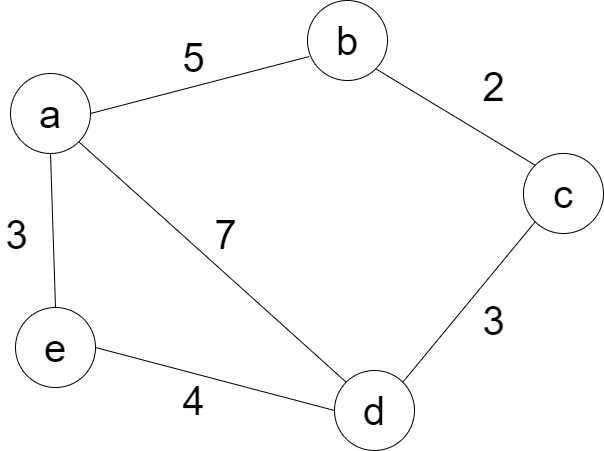
\includegraphics[width=\linewidth]{images/undirGraph.png}
		\caption{Ungerichteter gewichteter Graph}
		\label{fig:undirGraph}
	\end{minipage}
	\hfill
	\begin{minipage}[b]{0.45\textwidth}
		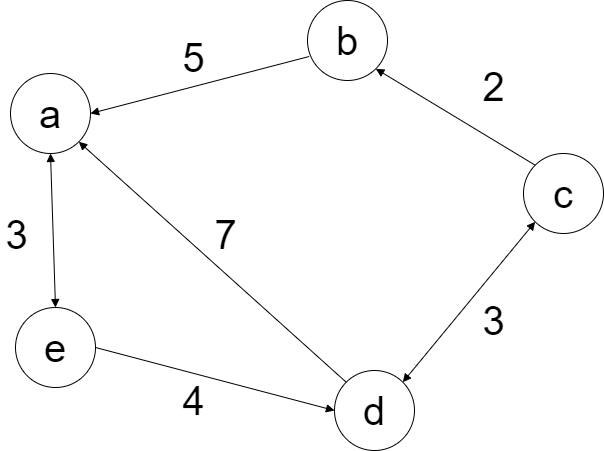
\includegraphics[width=\linewidth]{images/dirGraph.png}
		\caption{Gerichteter gewichteter Graph}
		\label{fig:dirGraph}
	\end{minipage}
\end{figure}

Zum Lösen des Problems des kürzesten Pfades in einem Graphen werden Suchalgorithmen benutzt. Diese lassen sich in informierte und uninformierte Algorithmen unterteilen. Die beiden Gruppen werden im folgenden Kapitel näher besprochen.

